\documentclass[tikz]{standalone}
\usepackage{tikz}
\usepackage{ifthen}

\begin{document}
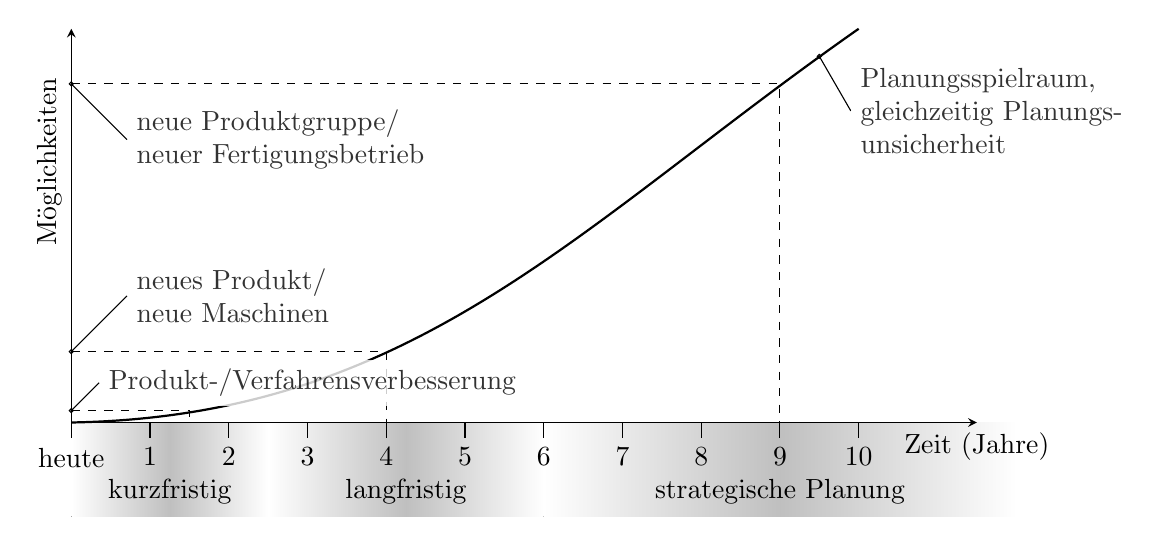
\begin{tikzpicture}[scale=1]



\fill[left color=white, right color=white, middle
        color=gray!50] (0,0) rectangle (2.5,-1.2) node[midway, below]{kurzfristig} ;
\fill[left color=white, right color=white, middle
        color=gray!50] (2.5,0) rectangle (6,-1.2) node[midway, below]{langfristig} ;
\fill[left color=white, right color=white, middle
        color=gray!50] (6,0) rectangle (12,-1.2) node[midway, below]{strategische Planung} ;



\draw[-stealth] (0,0)--(11.5,0)node[below]{Zeit (Jahre)};
\draw[-stealth] (0,0)--(0,5)node[sloped, above left, pos=.9]{Möglichkeiten};

\foreach \x in {0,1,...,10}{
\ifthenelse{0=\x}{\def\te{heute}}{\def\te{\x}}
\draw(\x,0)--++(0,-.2)node[below]{\te};
}


\draw[thick] (0,0)to[out=1, in = 215] (10,5);

\begin{scope}[dashed]


\draw (0,.9)coordinate(x)-|(4,0);
\draw[solid] (x)circle(.025)--++(45:1)node[right,fill=white,opacity=.8,align=left]{neues Produkt/ \\ neue Maschinen};


\draw (0,.15)coordinate(x)-|(1.5,0);
\draw[solid] (x)circle(.025)--++(45:.5)node[right,fill=white,opacity=.8]{Produkt-/Verfahrensverbesserung};

\draw (0,4.3)coordinate(x)-|(9,0);
\draw[solid] (x)circle(.025)--++(-45:1)node[right,fill=white,opacity=.8,align=left]{neue Produktgruppe/ \\ neuer Fertigungsbetrieb};

\draw[solid] (9.5,4.65)circle(.025)--++(-60:0.8)node[right,fill=white,opacity=.8,align=left]{Planungsspielraum, \\ gleichzeitig Planungs- \\ unsicherheit};


\end{scope}

\end{tikzpicture}
\end{document}